\lecture{4}{5. Februar 2025}{Imperfections in solids}

\section{Solidification}
The subject of today is imperfections in solids and therefore it is important to also mention solidification. A typical solidification follows this process
\begin{enumerate}
  \item \textbf{Molecular motion in the liquid} \\
    In the liquid state, molecules and/or atoms have relatively high kinetic energies and they move freely in a disordered manner. The high kinetic energy of the atoms/molecules keeps them from settling into position and establishing long-range order.
  \item \textbf{Cooling and reduction in kinetic energy} \\
    As the liquid cools the kinetic energy of the atoms/molecules decreases. This smaller amount of energy means that the attractive intermolecular/interatomic forces can begin to dominate. This slowly pulls the atoms/molecules more together and slowly establishes order.
  \item \textbf{Nucleation:} \\
    When the kinetic energy of the atoms/molecules has become small enough small clusters of atoms or molecules will start to come together. Sometimes these form spontaneously in the bulk liquid -- a process referred to as \textit{homogeneous nucleation}. Often, impurities, container walls or other surfaces provide a point of nucleation -- this if referred to as \textit{heterogeneous nucleation}. It should also be noted that not all small clusters will grow into a solid crystal. Each nucleus must reach a size where it is thermodynamically stable, meaning that the amount of energy gained from forming a solid outweighs the energy cost of creating a new interface between the solid and the liquid.
  \item \textbf{Crystal growth} \\
    Once a stable nucleus has formed, additional molecules/atoms from the liquid will start to attach to it. Molecules/atoms will approach the nucleus and if their orientation and energy is correct they will attach to the nucleus. This process is highly directional as molecules will align themselves in a pattern that reflects the symmetry and spacing of the crystal lattice. This process will (always?) release some latent heat, which can raise the temperature of the crystal and the surrounding liquid if the heat, for some reason, is not effectively removed.
  \item \textbf{Role of impurities} \\
    During the solidification process impurities can be introduced. Impurities are either incorporated or rejected from the crystal lattice based on their chemical compatibility with the host lattice. If an impurity does not fit well inside the lattice, it will tend to accumulate at an interface between the liquid and solid phases. If too much impurity accumulates here it can affect the growth of the crystals.
  \item \textbf{Completion of solidification} \\
    As more and more molecules are organized into a crystal lattice the entire volume of the liquid will soon have turned solid. Many of the final properties of the solid -- such as grain size, defect density, and impurity distribution -- are determined by the conditions during solidification. 
\end{enumerate}
This entire process is also shown briefly in \textbf{\autoref{fig:f4_1}}.
\begin{figure} [ht]
  \centering
  \caption{Solidification process}
  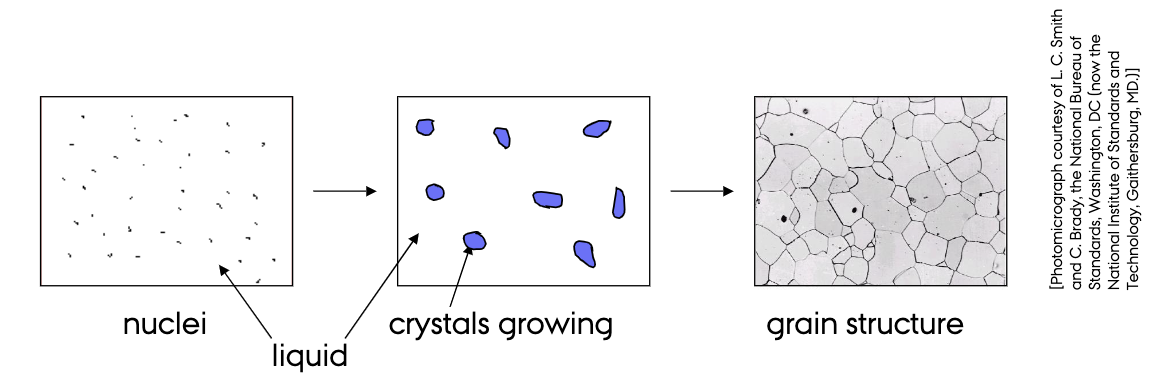
\includegraphics[width=0.75\linewidth]{./figures/f4_1.png}
  \label{fig:f4_1}
\end{figure}
As mentioned in part 6. of the solidification process explanation some of the properties of the solidified solid are determined by the conditions of the solidification process. This is explained a bit below.
\begin{itemize}
  \item \textbf{Types of Grains:}
    \begin{itemize}
      \item \textbf{Equiaxed Grains:} \\
        These grains are approximately equal in all directions. They typically form under rapid cooling conditions, where many nuclei form simultaneously. The fast extraction of heat limits their growth, resulting in a fine, isotropic grain structure (see \textbf{\autoref{fig:f4_2}}).
      
      \item \textbf{Columnar Grains:} \\
        These are elongated grains that grow predominantly in one direction, often aligned with the heat flow. When cooling is slower, nucleation is limited and existing grains have more time to grow directionally, resulting in a columnar structure (see \textbf{\autoref{fig:f4_2}}).
    \end{itemize}
  
  \item \textbf{Heat Flow and Cooling Rate:}
    \begin{itemize}
      \item \textbf{Rapid Cooling Near the Walls:} \\
        The outer regions of a casting, for example, cool more quickly due to heat extraction toward the mold walls. This rapid cooling promotes a high nucleation rate and the formation of many small, equiaxed grains.
      
      \item \textbf{Slower Cooling in the Center:} \\
        The interior of the material cools more slowly, allowing directional solidification. This slower rate favors the growth of fewer, larger columnar grains aligned with the heat flow.
    \end{itemize}
  
  \item \textbf{Role of Grain Refiners:} \\
    Additives known as grain refiners can be used to promote the formation of smaller, more uniform equiaxed grains. These refiners provide additional nucleation sites and help disrupt the growth of large columnar grains, which is often desirable for improving isotropy and mechanical properties. In many ways one can think of the fact that it is easier to make it ``random'' each time and thus rely on the law of large numbers to determine the properties than to rely on making exactly the same type of large columnar grains each time.
  
  \item \textbf{Real-World Implications:} \\
    In cast metals and alloys, the combination of equiaxed and columnar grains can have a significant impact on mechanical properties. Equiaxed grains typically enhance toughness and isotropy, while columnar grains may introduce anisotropy that is either beneficial or detrimental depending on the application.
\end{itemize}
\begin{figure} [ht]
  \centering
  \caption{Example of different grain types due to different solidification conditions.}
  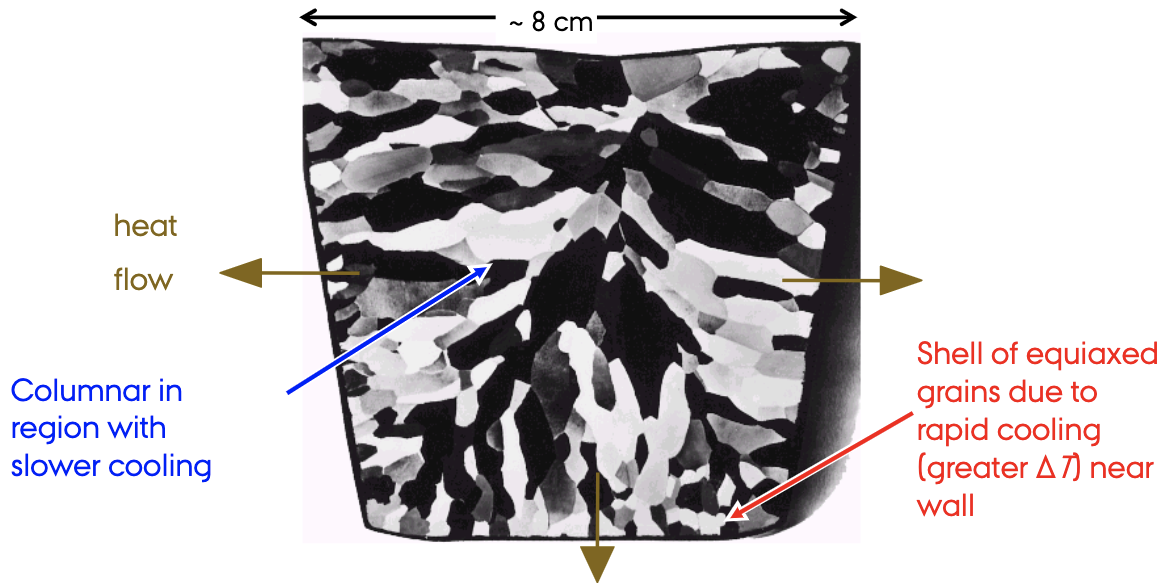
\includegraphics[width=0.65\linewidth]{./figures/f4_2.png}
  \label{fig:f4_2}
\end{figure}

\section{Imperfections}
There is no such thing as a perfect crystal -- crystalline imperfections (or \textit{defects}) are always present. This detail is not merely trivial as many important properties of materials are rather sensitive to defects. 

\subsection{Types of imperfections}
A few common types of imperfections will be explained in the next few paragraphs. These are
\begin{itemize}
  \item Point defects (0-dimensional)
    \begin{itemize}
      \item Vacancies
      \item Interstitial atoms
      \item Substitutional impurity atoms
    \end{itemize}
  \item Linear defects (1-dimensional)
    \begin{itemize}
      \item Dislocations
    \end{itemize}
  \item Interfacial defects (2-dimensional)
    \begin{itemize}
      \item Grain boundaries
    \end{itemize}
\end{itemize}

\subsection{Point defects}

\subsubsection{Vacancies}
\begin{itemize}
  \item \textbf{Definition:} \\
    A vacancy is a point defect where an atom is missing from one of the regular lattice sites. Imagine the perfect crystal lattice as a grid of atoms—if one atom is absent, a vacancy is created (see \textbf{\autoref{fig:f4_3}}).
  \item \textbf{Formation:} \\
    Vacancies can form during the crystallization process or be introduced thermally when atoms gain enough energy to leave their lattice sites. The equilibrium concentration of vacancies increases with temperature. The equilibrium concentration of vacancies for a given material and temperature is given by
    \[ 
    \frac{N_v}{N} = e^{-\frac{Q_v}{kT}}
    .\]
    Where $N_v$ is the amount of vacancies, $N$ is the amount of lattice positions (maximum amount of vacancies), $Q_v$ is the activation energy for forming a vacancy, $k$ is Boltzmann's constant and $T$ is the absolute temperature. The activation energy for forming a vacancy $Q_v$ is material and crystal structure specific and must be determined experimentally. 
  \item \textbf{Effects on Material Properties:}
    \begin{itemize}
      \item \textbf{Diffusion:} Vacancies facilitate atomic diffusion. Atoms can "jump" into adjacent vacant sites, allowing mass transport through the lattice.
      \item \textbf{Mechanical Properties:} A high concentration of vacancies can weaken the material by providing sites for crack initiation or influencing creep behavior
      \item \textbf{Electrical Properties:} In semiconductors, vacancies can act as electron traps, affecting conductivity.
    \end{itemize}
\end{itemize}
\begin{figure} [ht]
  \centering
  \caption{Vacancy in a crystal lattice}
  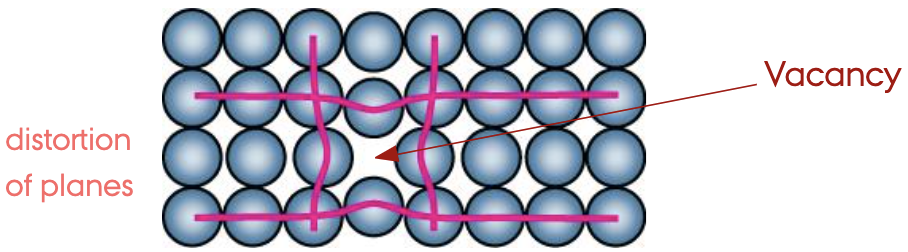
\includegraphics[width=0.65\linewidth]{./figures/f4_3.png}
  \label{fig:f4_3}
\end{figure}


\subsubsection{Interstitials} \label{sec:interstitial}
\begin{itemize}
  \item \textbf{Definition:} \\
    An interstitial defect occurs when an extra atom occupies a space (an interstice) between the regular lattice sites. These positions are normally empty in an ideal crystal (see \textbf{\autoref{fig:f4_4}}).
  \item \textbf{Types of Interstitial Atoms}
    \begin{itemize}
      \item \textbf{Host atoms:} Sometimes atoms from the same element may become interstitials if they are displaced from their normal lattice sites.
      \item \textbf{Impurity atoms:} Foreign atoms, often smaller than the host atoms, can fit into the interstitial spaces.
    \end{itemize}
  \item \textbf{Effects on Material Properties:}
    \begin{itemize}
      \item \textbf{Strain and Distortion:} Because an interstitial atom does not fit perfectly into the lattice, it can distort the surrounding atomic arrangement, leading to local stress.
      \item \textbf{Hardening:} In some metals, interstitial impurities (such as carbon in iron to form steel) increase the material’s hardness by impeding dislocation movement.
      \item \textbf{Diffusion:} Similar to vacancies, interstitial atoms can enhance diffusion; however, their movement mechanisms and activation energies differ from those of vacancies.
    \end{itemize}
\end{itemize}
\begin{figure} [ht]
  \centering
  \caption{Interstitial defect in a crystal lattice}
  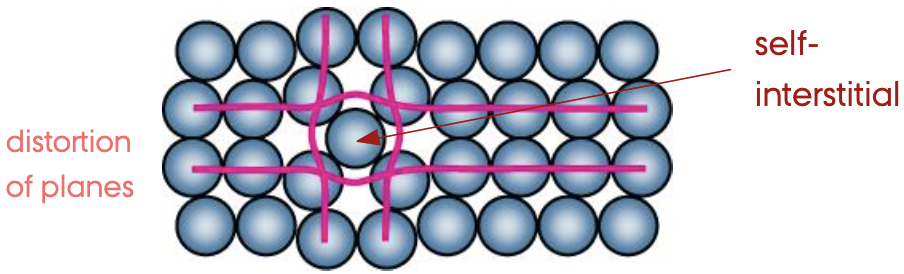
\includegraphics[width=0.65\linewidth]{./figures/f4_4.png}
  \label{fig:f4_4}
\end{figure}



\subsubsection{Substitutional Impurity Atoms} \label{sec:substitutional}
\begin{itemize}
  \item \textbf{Definition:} \\
    A substitutional impurity occurs when an atom of a foreign element takes the place of a host atom in the crystal lattice. This defect is "substitutional" because the impurity substitutes for a lattice atom (see \textbf{\autoref{fig:f4_5}}).
  \item \textbf{Formation:}
    \begin{itemize}
      \item \textbf{During Solidification:} Substitutional impurities can become incorporated into the lattice as the material solidifies from the liquid state if the impurity atoms are present in the melt.
      \item \textbf{Doping Processes:} In semiconductors, substitutional doping is intentionally carried out to modify electrical properties by replacing some host atoms with impurity atoms that have different valence electron configurations.
    \end{itemize}
  \item \textbf{Effects on Material Properties:}
    \begin{itemize}
      \item \textbf{Mechanical Properties:} The presence of substitutional impurities can distort the lattice due to differences in atomic size compared to the host atoms. This distortion can either strengthen the material (by impeding dislocation movement) or weaken it if excessive strain is introduced.
      \item \textbf{Electrical Properties:} In semiconductors, substitutional impurities are crucial for controlling conductivity. For example, replacing a silicon atom with a phosphorus atom (which has five valence electrons) creates an excess of electrons ($n$-type doping), whereas using boron (with three valence electrons) results in $p$-type doping by creating holes.
      \item \textbf{Thermal Properties:} The lattice distortion and scattering of phonons by impurity atoms can affect the thermal conductivity of the material.
      \item \textbf{Chemical properties:} The chemical reactivity may also be altered if the impurity atoms interact differently with the environment compared to the host atoms.
    \end{itemize}
\end{itemize}
\begin{figure} [ht]
  \centering
  \caption{Substitutional impurity in a crystal lattice}
  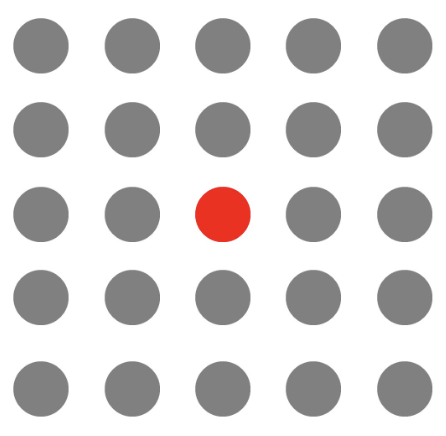
\includegraphics[width=0.3\linewidth]{./figures/f4_5.png}
  \label{fig:f4_5}
\end{figure}

\begin{exa}[Equilibrium number of vacancies in 1 cubic meter of copper at 1000 degrees celsius]
  We want to determine the equilibrium number of vacancies in \qty{1}{m^3} Cu at \qty{1000}{\celsius}.
  \bigbreak
  We start by finding the total amount of lattice sites using the formula
  \[ 
  N = \frac{N_A \rho}{A}
  .\]
  Where $N_A$ is Avogadro's constant, $\rho$ is the density of the material and $A$ is the atomic weight. By substituting in known values we get
  \[ 
    N = \frac{\qty{6,022e23}{mol^{-1}} \cdot \qty{8,4}{\frac{g}{cm^3}}}{\qty{63,5}{\frac{g}{mol}}} = \qty{8,0e28}{mol^{-1}} 
  .\]
  We can now determine the equilibrium number of vacancies as
  \[ 
  N_v = N e^{- \frac{Q_v}{k T}}
  .\]
  $Q_v$ has experimentally been found to be $Q_v = \qty{0,9}{eV}$ for Cu and thus we get
  \[ 
  N_v = N e^{-\frac{\qty{0,9}{eV}}{\qty{8,62e-5}{\frac{eV}{K}} \cdot \qty{1273}{K}}} = \left( \num{2,7e-4}  \right)N = \qty{2,2e25}{m^{-3}} 
  .\]
  I.e. we expect there to be \qty{2,2e25}{m^{-3}} vacancies in \qty{1}{m^3}  of Cu. 
\end{exa}

\begin{exa}[Calculation of fraction of vacancies]
  For some hypothetical metal the equilibrium number of vacancies at \qty{900}{\celsius} is \qty{2,3e25}{m^{-3}}. If the density and atomic weights are \qty{7,40}{g/cm^3} and \qty{85,5}{g/mol}, respectively, calculate the fraction of vacancies for this metal at \qty{900}{\celsius}.
  \bigbreak
  We can use the same formula for the amount of lattice positions as we did above
  \[ 
  N = \frac{N_A \rho}{A} = \frac{\qty{6,022e23}{mol^{-1}} \cdot \qty{7,40}{\frac{g}{cm^3}}}{\qty{85,5}{\frac{g}{mol}}} = \qty{5,21e28}{m^{-3}}
  .\]
  Now we can find the fraction as
  \[ 
    \frac{N_v}{N} = \frac{\qty{2,3e25}{m^{-3}}}{\qty{5,21e28}{m^{-3}}} = \num{4,41e-4}
  .\]
\end{exa}

\subsubsection{Impurities in metals}
If impurity atoms are added to a solid composed of host atoms then the impurities will start to dissolve into the host lattice. Until the impurity concentration exceeds the solubility limit the impurities will simply dissolve into the main metal. After exceeding the solubility limit no more impurity can be dissolved into the main metal. Instead a ``secondary phase'' is formed which can have a different structure than the main metal. This secondary phase will also build grains in the same way the primary phase (main metal) does.

A few different rules dictate how impurities can be added to metals. These are known as the Hume-Rothery rules. There are two sets of Hume-Rothery rules -- one for substitutional solid solutions and one for interstitial solid solutions. These are

\paragraph{Hume-Rothery Rules for Substitutional Solid Solutions}
\begin{enumerate}
  \item The atomic radius of the solute and solvent must differ by no more than 15\%.
  \item The crystal structures of the solvent and solute must be similar.
  \item Complete solubility occurs when the solvent and solute have the same valency. A metal is more likely to dissolve a metal of higher valency, than vice versa.
  \item The solute and solvent should have similar electronegativity. If the electronegativity difference is too great, the metals tend to form intermetallic compounds instead of solid solutions.
\end{enumerate}

\paragraph{Hume-Rothery Rules for Interstitial Solid Solutions}
\begin{enumerate}
  \item Solute atoms should have a smaller radius than 59\% of the radius of solvent atoms.
  \item The solute and solvent should have similar electronegativity.
  \item The solute and solvent should have the same valence. The greater the difference in valence between solute and solvent atoms, the lower the solubility.
\end{enumerate}

\begin{exa}[Application of the Hume-Rothery Rules]
  We want to determine whether Al or Ag is more likely to form a substitutional solid solution in Zn.
  \bigbreak
  The atomic radii are $r_{Zn} = \qty{0,1332}{nm}$, $r_{Al} = \qty{0,1431}{nm}$ and $r_{Ag} = \qty{0,1445}{nm}$. It can be observed, that in terms of difference of atomic radii, Al is slightly favoured compared to Ag.

  The crystal structures for both Al and Ag are FCC, whereas it is HCP for Zn. This means Al and Ag are tied for this criterion.

The valence of Ag is +1, for Al it is +3 and for Zn it is +2. As the valence of Al $>$ Ag this criterion favors Al.

  The electronegativity of Zn is \num{1,6}, whilst it is \num{1,9} and \num{1,5} for Ag and Al, respectively. As the electronegativity of Al is closer to Zn than the electronegativity of Ag is, Al must be favored in this criterion as well.

  Based on the above it seems more likely that Al will form a substitutional solid solution in Zn than that Ag will.
\end{exa}

\subsection{Linear defects}
All linear defects are examples of \textit{dislocations}. These are 1-dimensional defects around which atoms are misaligned. However to really understand these we first need to introduce the concept of \textit{Burger's vector}, $\Vec{b}$.

\subsubsection{Burger's vector}
The Burger's vector, $\Vec{b}$, is a vector that represents both the magnitude and the direction of the lattice distortion caused by a dislocation. It essentially quantifies the ``missing'' or ``extra'' displacement in the crystal lattice due to the dislocation. To determine the magnitude and direction of Burger's vector one must follow this procedure:
\begin{enumerate}
  \item Visualize the crystal structure without the defect, i.e. the \textit{perfect} crystal structure.
  \item Construct a rectangle encompassing the site of the dislocation with side lengths that are integer multiples of $a$ (the edge length of the UC). This rectangle is known as a \textit{Burger's circuit}-
  \item Reintroduce the dislocation in the visualization.
  \item The, previously closed, Burger's circuit will know have been deformed along with the crystal lattice underneath. The ``missing'' vector that is needed to close the loop is then the Burger's vector.
\end{enumerate}

\subsubsection{Edge Dislocations}
\begin{itemize}
  \item \textbf{Definition:} \\
    An edge dislocation is a line defect in a crystal lattice characterized by the presence of an extra half-plane of atoms that terminates within the crystal. This extra half-plane creates a localized distortion of the surrounding lattice (see \textbf{\autoref{fig:f4_6}}).
  \item \textbf{Formation:} \\
    Edge dislocations can form during processes such as plastic deformation, where the crystal is subjected to stresses that force an extra half-plane of atoms into the lattice, or due to thermal stresses. The introduction of these dislocations helps accommodate the strain imposed on the crystal.
  \item \textbf{Burgers Vector:} \\
    The magnitude and direction of the lattice distortion are described by the Burgers vector. For an edge dislocation, the Burgers vector is perpendicular to the dislocation line, quantifying the shift of atomic planes relative to each other.
  \item \textbf{Effects on Material Properties:}
    \begin{itemize}
      \item \textbf{Plastic Deformation:} \\
        The movement of edge dislocations under applied stress allows layers of atoms to slip past each other, which is the primary mechanism for permanent (plastic) deformation in crystalline materials.
      \item \textbf{Work Hardening:} \\
        As deformation progresses, the density of dislocations increases and they interact with one another. These interactions can impede further dislocation movement, thereby increasing the strength of the material through work hardening.
      \item \textbf{Stress Concentration:} \\
        The localized lattice distortion around an edge dislocation creates regions of high internal stress. These stress concentrations can act as initiation sites for cracks, influencing the material's fracture behavior.
    \end{itemize}
\end{itemize}

\begin{figure}[ht]
  \centering
  \caption{Edge dislocation in a crystal lattice}
  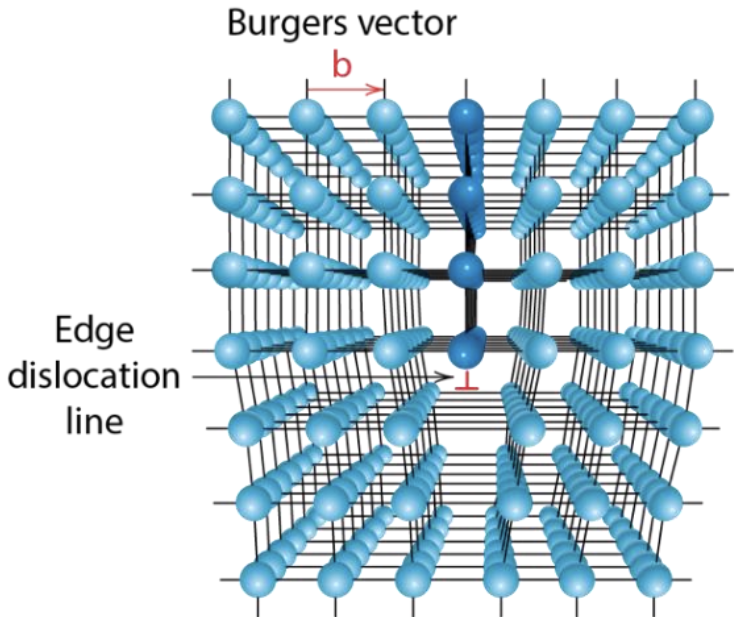
\includegraphics[width=0.35\linewidth]{./figures/f4_6.png}
  \label{fig:f4_6}
\end{figure}


\subsubsection{Screw Dislocations}
\begin{itemize}
  \item \textbf{Definition:} \\
    A screw dislocation is a line defect in a crystal lattice characterized by a helical arrangement of the atomic planes around the dislocation line. Unlike an edge dislocation, a screw dislocation does not have an extra half-plane of atoms; instead, the lattice shifts in a spiral manner around the defect (see \textbf{\autoref{fig:f4_7}}).
  \item \textbf{Formation:} \\
    Screw dislocations are commonly formed during plastic deformation when shear stresses are applied to the crystal. These stresses cause the atomic planes to shift relative to one another in a helical path, creating the screw dislocation.
  \item \textbf{Burgers Vector:} \\
    In the case of a screw dislocation, the Burgers vector is parallel to the dislocation line.
  \item \textbf{Effects on Material Properties:}
    \begin{itemize}
      \item \textbf{Plastic Deformation:} The motion of screw dislocations under applied stress enables shear deformation of the crystal, contributing to the material's overall ductility.
      \item \textbf{Dislocation Mobility:} Screw dislocations can move through the lattice via a process called \textit{glide} (along specific crystallographic planes) or \textit{climb} (perpendicular to the glide plane, often assisted by diffusion), affecting the rate and mode of deformation.
      \item \textbf{Interaction with Other Defects:} The presence of screw dislocations influences the interaction with other dislocations and defects, which can either facilitate or impede further movement and thus impact the work hardening and strength of the material.
    \end{itemize}
\end{itemize}

\begin{figure}[ht]
  \centering
  \caption{Screw dislocation in a crystal lattice}
  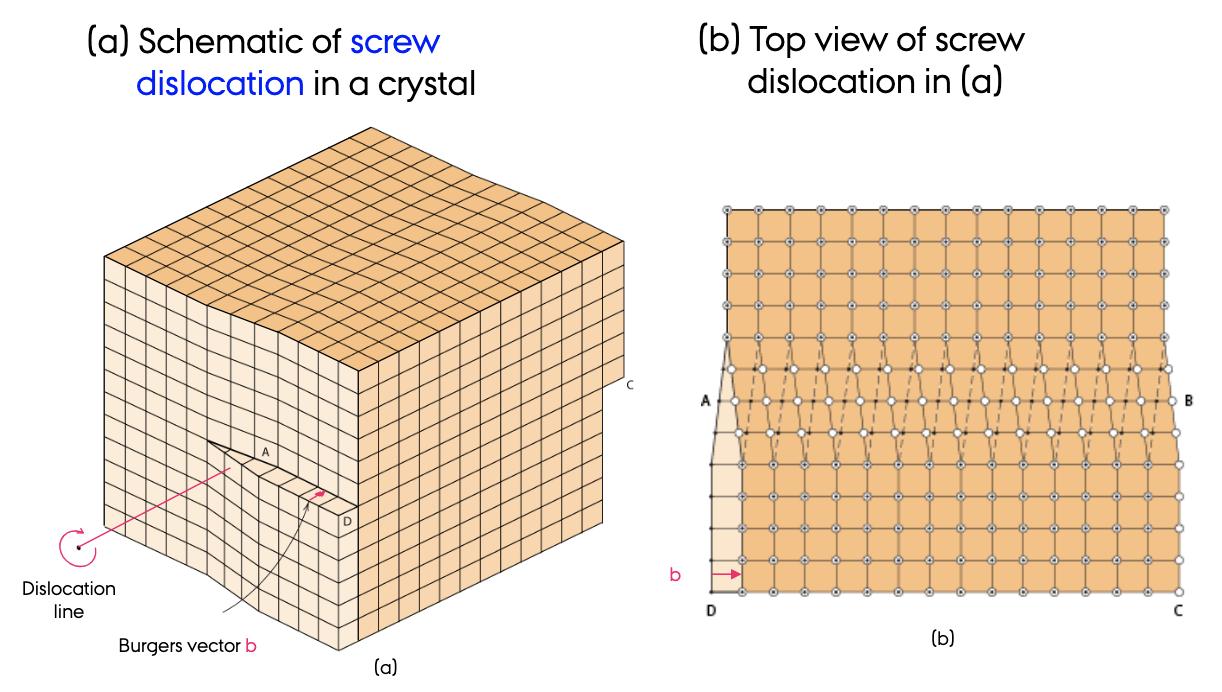
\includegraphics[width=0.55\linewidth]{./figures/f4_7.png}
  \label{fig:f4_7}
\end{figure}


\subsubsection{Mixed Dislocations}
\begin{itemize}
  \item \textbf{Definition:} \\
    Mixed dislocations are line defects in the crystal lattice that possess both edge and screw components. The dislocation line in these cases does not lie entirely in the plane of the extra half-plane (as in a pure edge dislocation) nor is it completely parallel to the Burgers vector (as in a pure screw dislocation) (See \textbf{\autoref{fig:f4_8}}).
  \item \textbf{Characteristics:} \\
    The local character of a mixed dislocation may vary along its length, with certain segments behaving more like edge dislocations and others more like screw dislocations.
  \item \textbf{Importance:} \\
    Most dislocations in real materials are mixed, and their complex behavior influences the material's plastic deformation, work hardening, and interaction with other defects.
\end{itemize}

\begin{figure} [ht]
  \centering
  \caption{Mixed dislocation in a crystal lattice}
  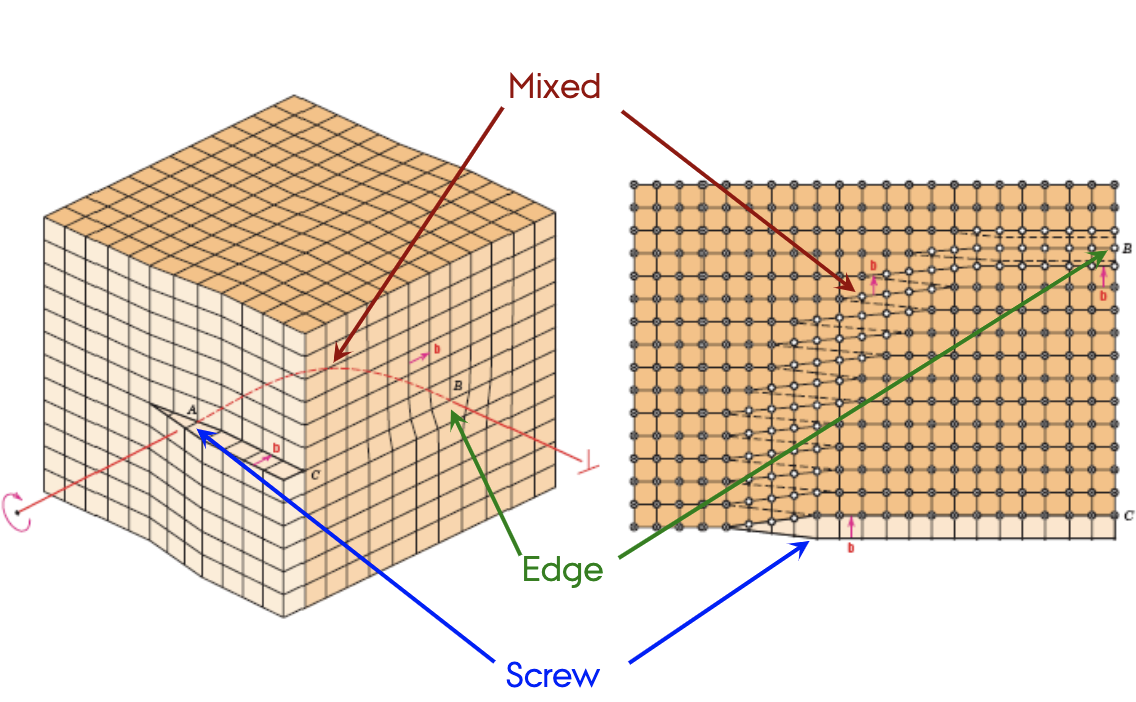
\includegraphics[width=0.5\linewidth]{./figures/f4_8.png}
  \label{fig:f4_8}
\end{figure}

\subsubsection{Plastic deformation and dislocations}
When an external stress is applied to a material dislocations will begin to move. As these dislocations move through the material they allow layers of atoms to slip relatively to each other. This is what leads to plastic deformation. The fact that dislocations can move under applied stress is central to the idea of ductility in many materials.  In a single crystal metal, when dislocations move to the surface, they leave behind small steps. Each step corresponds to a dislocation slip event. These incremental steps collectively account for the overall plastic deformation of the material. This mechanism is shown in \textbf{\autoref{fig:f4_9}}. Based on the above it is clear that plastic deformation is not a smooth, continuous process but rather the accumulation of many discrete events. Each time a dislocation moves and reaches the surface, it produces a step. Over time, these steps add up, leading to a measurable change in shape of the material.
\begin{figure} [ht]
  \centering
  \caption{Plastic deformation in a single-crystal metal}
  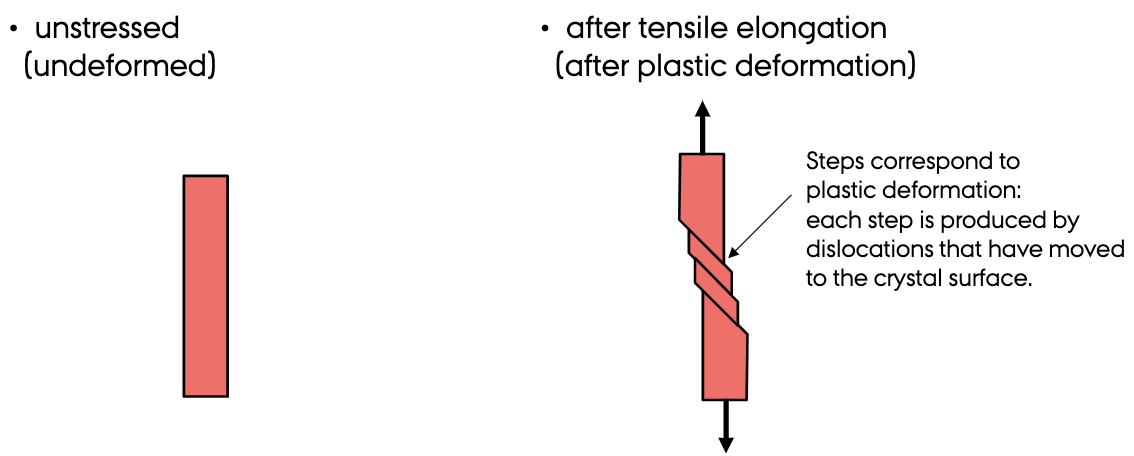
\includegraphics[width=0.75\linewidth]{./figures/f4_9.png}
  \label{fig:f4_9}
\end{figure}

\subsection{Planar defects}
\subsubsection{Twin Boundaries}
\begin{itemize}
  \item \textbf{Definition:} \\
    A twin boundary is a planar defect where two adjacent regions of a crystal are mirror images of each other across a specific crystallographic plane. This mirror symmetry distinguishes twin boundaries from other types of interfaces in the crystal (see \textbf{\autoref{fig:f4_10}}).
  \item \textbf{Formation:} \\
    Twin boundaries can form during:
    \begin{itemize}
      \item \textbf{Crystal Growth:} During solidification or annealing, certain conditions may favor the formation of twin domains.
      \item \textbf{Plastic Deformation:} Under high strain rates or low temperatures, deformation twins may form as a mechanism to accommodate plastic deformation.
    \end{itemize}
  \item \textbf{Effects on Material Properties:}
    \begin{itemize}
      \item \textbf{Strengthening Mechanism:} Twin boundaries can impede dislocation motion, which may enhance the material’s strength.
      \item \textbf{Toughness:} In some cases, twin boundaries can increase ductility and toughness by providing additional pathways for deformation.
      \item \textbf{Anisotropy:} The mirror symmetry may influence the directional properties of the material, leading to anisotropic behavior.
    \end{itemize}
\end{itemize}

\begin{figure}[ht]
  \centering
  \caption{Twin boundary in a crystal lattice}
  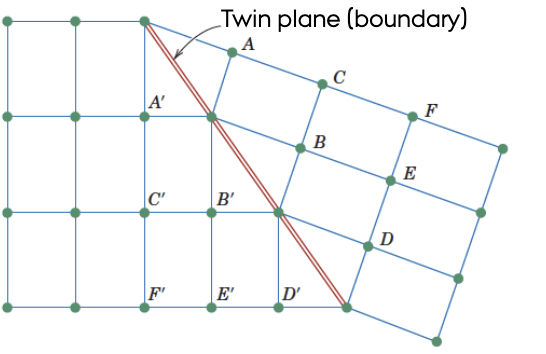
\includegraphics[width=0.45\linewidth]{./figures/f4_10.png}
  \label{fig:f4_10}
\end{figure}


\subsubsection{Grain Boundaries}
\begin{itemize}
  \item \textbf{Definition:} \\
    A grain boundary is the interface between two individual grains within a polycrystalline material, where the crystal lattice orientation changes abruptly. This boundary represents a discontinuity in the crystallographic arrangement (see \textbf{\autoref{fig:f4_11}}).
  \item \textbf{Formation:} \\
    Grain boundaries form during:
    \begin{itemize}
      \item \textbf{Solidification:} As a polycrystalline material cools, different grains nucleate and grow in various orientations. When these growing grains impinge upon one another, grain boundaries form.
      \item \textbf{Recrystallization:} During thermomechanical processing, new strain-free grains can nucleate within a deformed microstructure, resulting in new grain boundaries.
    \end{itemize}
  \item \textbf{Effects on Material Properties:}
    \begin{itemize}
      \item \textbf{Strengthening:} Grain boundaries act as barriers to dislocation motion, which increases strength. However, very small grains can also lead to a reduction in ductility.
      \item \textbf{Diffusion:} The less ordered structure at grain boundaries allows for enhanced diffusion compared to the crystal interior.
      \item \textbf{Corrosion and Creep:} Grain boundaries can serve as preferred sites for corrosion attack or creep deformation due to their higher energy and susceptibility to impurity segregation.
    \end{itemize}
\end{itemize}

\begin{figure}[ht]
  \centering
  \caption{Grain boundary in a polycrystalline material}
  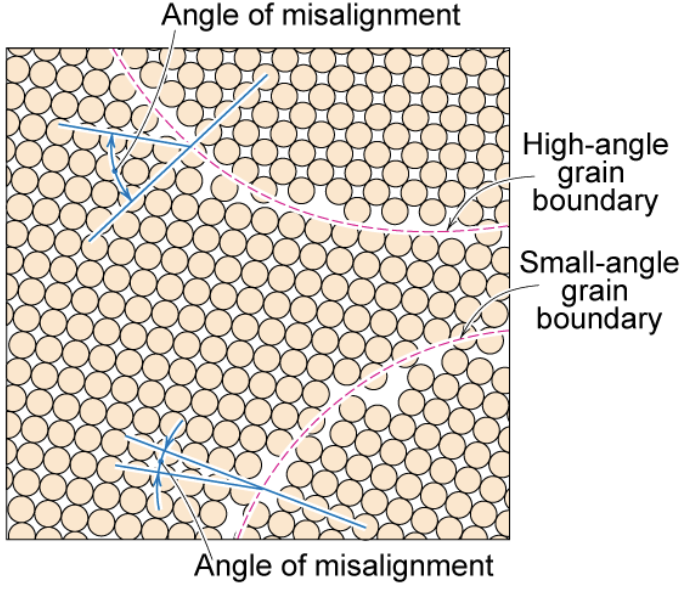
\includegraphics[width=0.35\linewidth]{./figures/f4_11.png}
  \label{fig:f4_11}
\end{figure}

\subsubsection{Stacking Faults}
\begin{itemize}
  \item \textbf{Definition:} \\
    A stacking fault is a planar defect that occurs when there is a disruption in the regular stacking sequence of atomic planes in a crystal. In close-packed structures, atoms are arranged in a specific order (e.g., ABCABC... in face-centered cubic (FCC) crystals or ABAB... in hexagonal close-packed (HCP) crystals). A stacking fault introduces a deviation from this ideal sequence (see \textbf{\autoref{fig:f4_12}}).
  \item \textbf{Understanding Stacking:}
    \begin{itemize}
      \item In FCC metals, the close-packed planes follow an \textit{ABC} stacking sequence. Each letter represents a distinct position of the plane relative to the one below it. For example, if the ideal stacking is ...ABCABCABC..., a fault might produce a sequence like ...ABC\textbf{AA}CABC..., where the normal progression is interrupted.
      \item In HCP metals, the ideal stacking sequence is \textit{ABAB...}. A fault in this sequence might result in a local deviation, such as an extra A or B layer, leading to a disrupted stacking order.
      \item The stacking sequence is critical because it determines the overall symmetry and slip systems available in the crystal, thereby influencing the mechanical properties.
    \end{itemize}
  \item \textbf{Formation:} \\
    Stacking faults can be formed during:
    \begin{itemize}
      \item \textbf{Crystal Growth:} Imperfections during the deposition of atomic layers can lead to errors in the stacking sequence.
      \item \textbf{Plastic Deformation:} Dislocation movement, especially partial dislocations, can create stacking faults. For example, in FCC metals, the motion of a partial dislocation leaves behind a stacking fault in the slip plane.
      \item \textbf{Phase Transformations:} Changes in temperature or pressure may induce stacking faults during transformations between different crystal structures.
    \end{itemize}
  \item \textbf{Effects on Material Properties:}
    \begin{itemize}
      \item \textbf{Influence on Dislocation Motion:} Stacking faults can modify the way dislocations move through a crystal. In some cases, they can act as barriers that impede dislocation glide, contributing to strengthening. In other cases, they may facilitate the splitting of dislocations into partials.
      \item \textbf{Planar Defect Energy:} The energy associated with a stacking fault depends on the degree of disruption in the stacking order. Lower stacking fault energies tend to promote the formation of extended partial dislocations, which can enhance ductility by allowing more cross-slip.
      \item \textbf{Twinning and Deformation Mechanisms:} In certain materials, stacking faults are precursors to deformation twinning—a process that can contribute to plastic deformation. The local reordering of the stacking sequence may lead to twin formation, which influences the material's mechanical response.
    \end{itemize}
\end{itemize}

\begin{figure}[ht]
  \centering
  \caption{Ideal stacking for HCP and FCC crystals.}
  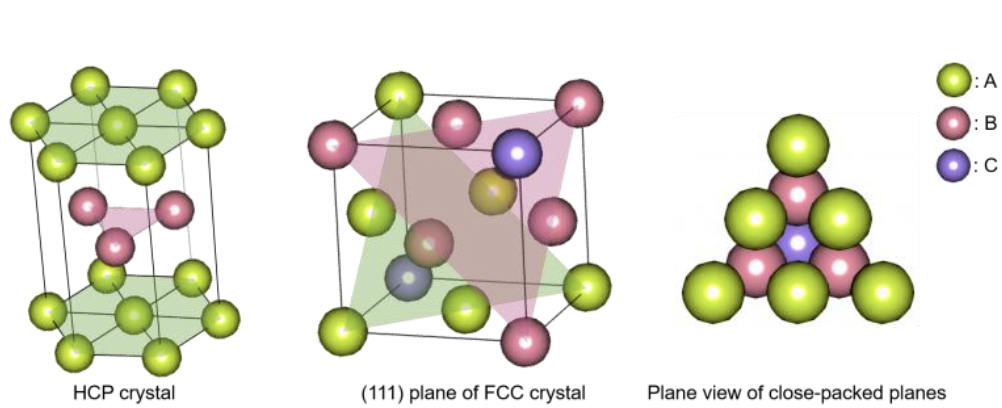
\includegraphics[width=0.65\linewidth]{./figures/f4_12.png}
  \label{fig:f4_12}
\end{figure}

